\chapter{动机、奖励和上瘾状态} \label{chap:chap43}

\section{动机状态影响目标导向的行为}

一天,一只猎豹躲在树荫下躲避正午的阳光,似乎对远处的羚羊漠不关心。
然而,下午稍晚时,看到羚羊会立即进行猎捕和潜伏的行为。
刺激是相同的,但行为反应却大不不同。
改变的是动物的动机状态。



动机状态影响注意力、目标选择、在追求目标中投入的努力以及对刺激的响应。
因此,它们驱动着接近、避免和行动选择。
本章重点关注与奖励相关的动机状态的神经生物学基础,以及奖励相关的脑回路如何参与了潜在的药物成瘾机制。



\subsection{内部和外部刺激都有助于激励状态}

动机状态反映一个人的欲望,而欲望会受到生理状态以及预测未来奖励和惩罚性事件刺激的影响。
因此,动机状态取决于内部和外部变量。
内部变量包括关于饥饿或口渴的生理信号,以及与生物钟相关的变量。
例如,觅食的频率和持续时间随一天中的时间、动物上次进食的时间以及雌性动物是否正在哺乳而变化。


其他内部变量与认知过程有关。
例如,在 21 点游戏中,同一张牌在不同的手中可能会导致玩家破产或获得 21 点,从而导致在随后的决策和行动选择中产生截然不同的情绪反应和调整。
对二十一点游戏规则的认知理解使得相同刺激(特定牌)的不同含义成为可能。
对规则的认知理解是一种内部变量。
同样,不同的社交场合常常会引发对同一刺激的不同行为反应,例如一个人是在大学聚会上大口喝酒还是在正式晚宴上啜饮。


外部变量也会影响动机状态。
这些变量包括奖励激励刺激。
例如,当一只脱水的猎豹在寻找羚羊的过程中遇到一个水坑时,看到水可能会起到激励作用,打破饥饿和口渴之间的平衡,驱使动物中断对食物和饮料的追求。
然而,一个内部变量(猎豹的水分状态)也可能导致不同的奖励值被分配给相同的感官刺激,即水坑。
即使是天生有益的刺激,例如通常会引起愉悦的甜味刺激物,在某些情况下也会变得令人不快。
巧克力蛋糕对巧克力爱好者来说可能是天生的奖励,但巧克力的饱腹感(涉及调节内部变量)会降低这种刺激的奖励价值,从而影响动机状态。



\subsection{奖励可以满足短期和长期的监管和非监管需求}

进食、饮水和体温调节行为及其潜在的动机状态通常是响应(或预期)生理失衡而出现的。
在这些情况下,行动会在相对较短的时间内获得奖励。
相比之下,一些动机状态服务于除了短期生理稳态之外的生理需要。
更复杂的长期目标,例如寻找和维持爱情伴侣或实现教育或职业目标,需要在更长的时间尺度上以目标为导向的行动。
非调节性动机状态可能类似于生理信号产生的动机状态,但动机行为通常涉及一系列行动,其中并非每一个行动都会立即得到奖励(除了在朝着长期目标取得进展的意义上)。


总的来说,激励性刺激,甚至是只表示向着长期目标迈进的刺激,都可以影响动机状态,从而完成复杂的行为序列。
这个概念的一个简单例子是,猎豹必须潜伏、追逐、追赶并杀死羚羊,然后拖着尸体到安全地带再开始进食。
当然,即使是觅食和进食所涉及的复杂动作,也远比有动机获得研究生学位和发展学术生涯的学生所需的步骤简单得多。
为了实现这些目标,必须在充满挑战的环境中维持激励状态。



\subsection{大脑的奖励回路为目标选择提供了生物基质}

奖励是具有积极价值的物品、刺激或活动。
奖励可以刺激动物从一种行为转变为另一种行为,或者抵制正在进行的行为的中断。
例如,一只老鼠在侦察环境时遇到种子可能会停止探索,以便吃掉种子或将其带到更安全的地方;
在啃种子时,老鼠会抵抗另一只老鼠从它的爪子上偷走食物的努力。
如果仅在特定位置和时间提供种子,老鼠将在预期的奖励发放时刻临近时前往该位置。


当代神经科学领域的许多工作都旨在阐明处理不同类型奖励的神经系统。
这些系统必须将奖励的初始感官表征与不同行为联系起来,以应对生理需求以及环境挑战和机遇。
成瘾等病态可以劫持这些奖励系统,导致适应不良行为(在本章后半部分讨论)。


以目标为导向的行为需要评估风险、成本和收益。
离开羚羊群可能会为羚羊提供更好的觅食机会,但这是以成为潜伏猎豹的目标为代价的。
攻击冒险的羚羊为猎豹提供了一个更容易进餐的承诺,但如果羚羊逃跑,能量和水资源可能会被不必要地消耗掉。
因此,负责目标选择的神经机制必须权衡可能实现特定目标的不同行为的成本和收益。


1954 年,\textit{詹姆斯$\cdot$奥尔兹}和\textit{米尔纳}报告了他们在负责奖励相关行为的神经通路方面的工作。
这些经典研究以脑电刺激为目标。
老鼠和从金鱼到人类的其他脊椎动物都会对某些大脑区域进行电刺激。
这种自我刺激的热情和持久性是显著的。
老鼠会穿过带电的电网,在跳过障碍的同时跑上坡,或者连续数小时按下控制杆以触发电刺激。
导致动物为自我刺激而工作的现象称为大脑刺激奖赏(图~\ref{fig:43_1}A)。
因此,大脑刺激会引发一种激励状态,一种执行将提供进一步刺激的动作(例如,杠杆按压)的强烈驱动力。


\begin{figure}[htbp]
	\centering
	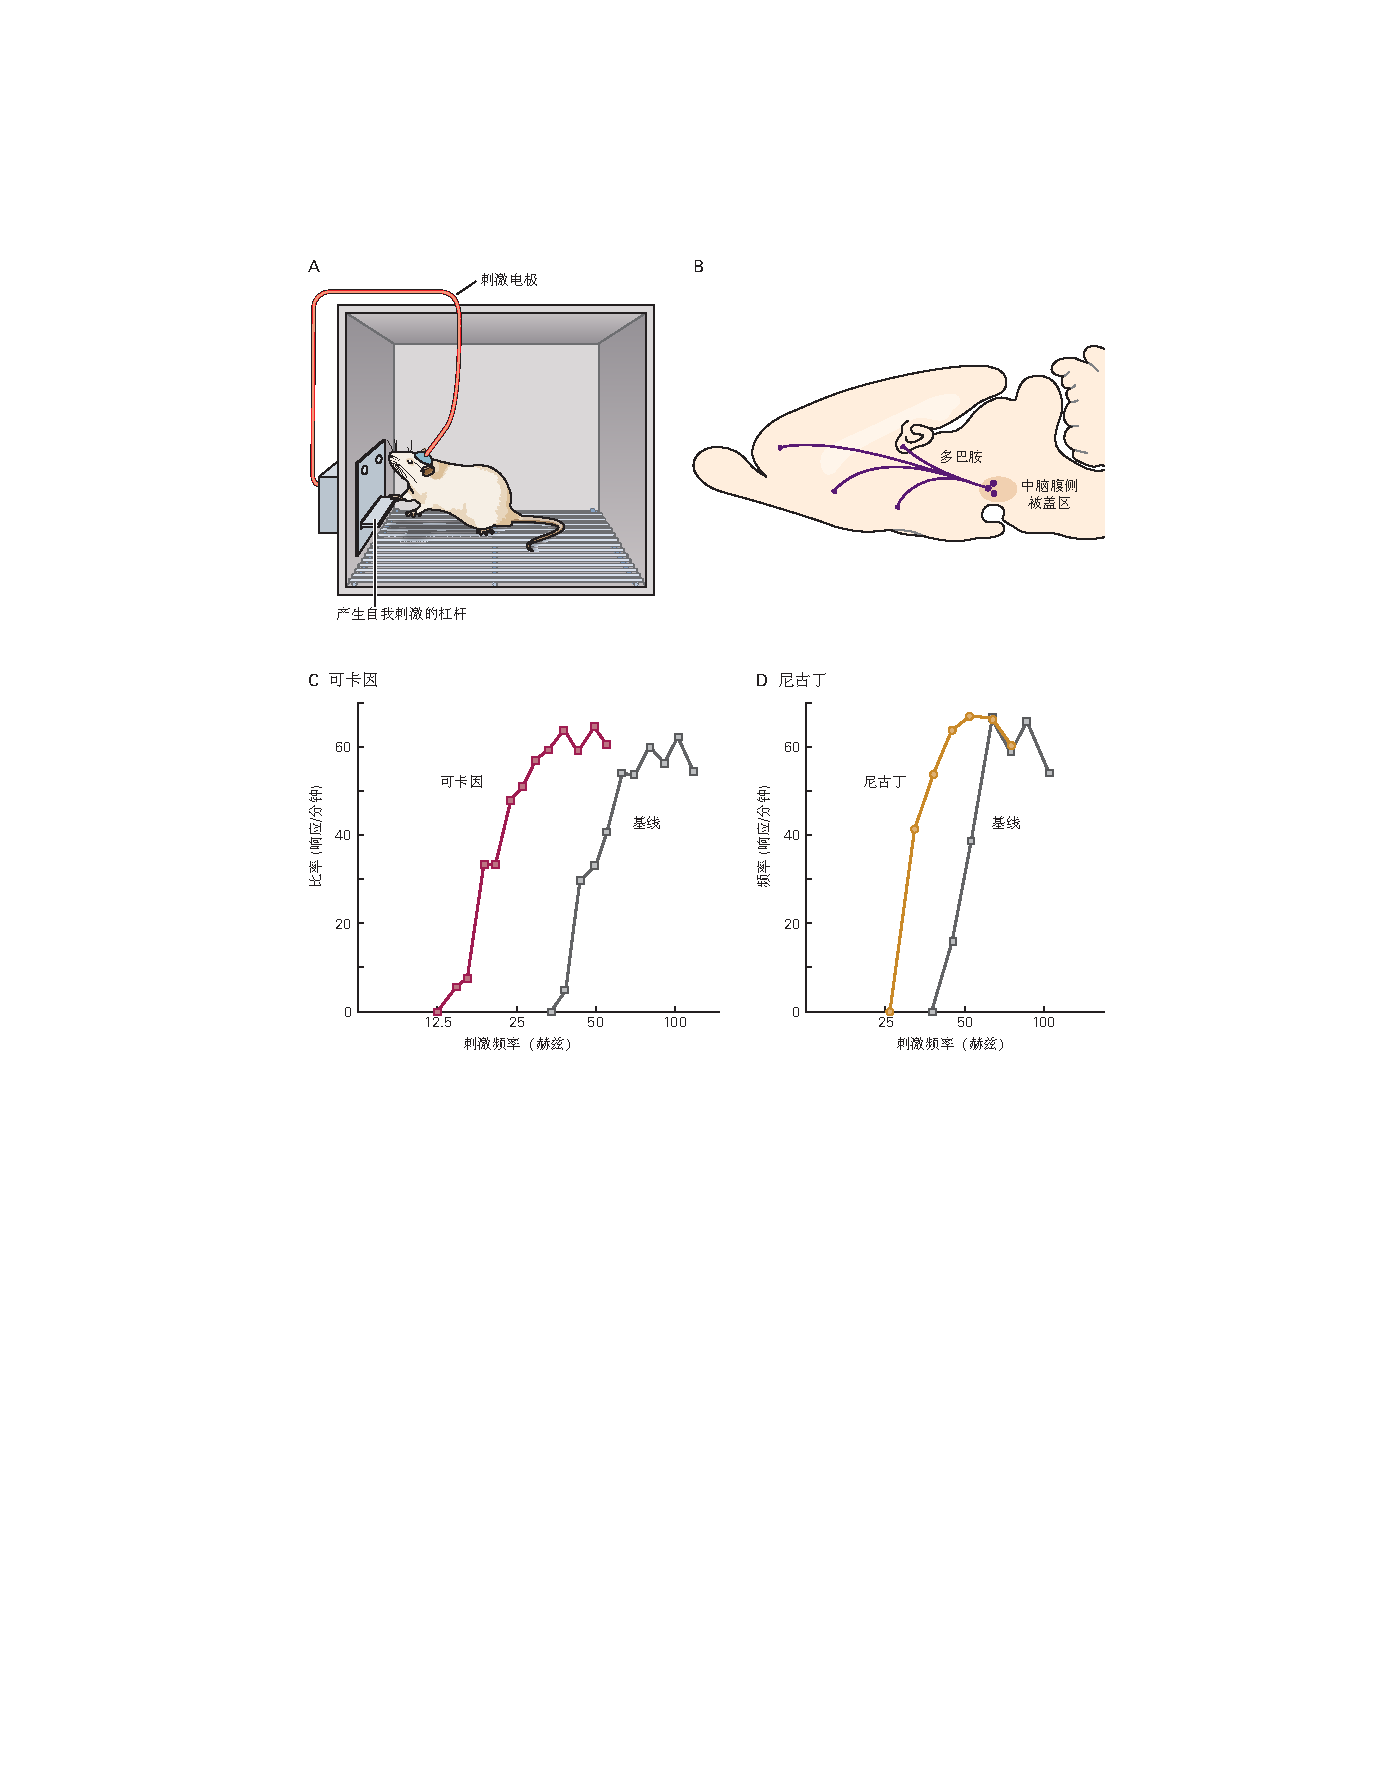
\includegraphics[width=0.9\linewidth]{chap43/fig_43_1}
	\caption{颅内自我刺激招募奖励回路和多巴胺能神经通路。
		\textbf{A.} 自刺激实验的经典测试仪器。
		在此示例中,电极被植入啮齿动物的大脑区域。
		啮齿动物按下杠杆会触发该大脑区域的电刺激。
		\textbf{B.} 产生自我刺激行为的大脑结构通常会激活从\textit{腹侧被盖区}发出的多巴胺能通路,以及其他通路。
		\textbf{C.D.} 可卡因和尼古丁会影响电自我刺激的速度。
		动物按压刺激杆的速率随着自我刺激电流频率的增加而增加。
		在药物存在的情况下,动物以较低的刺激频率按下控制杆,表明药物增强了电刺激的效果。}
	\label{fig:43_1}
\end{figure}


虽然大脑刺激奖励是一个人为的目标,但它模仿了自然目标对象的一些属性。
例如,大脑刺激可以与其他奖励预测刺激竞争、相加或替代,以诱导驱动目标导向行为的动机状态。
介导大脑刺激奖励的回路分布广泛。
奖励效应可以通过电刺激大脑各个层面的部位产生,从嗅球到孤束核。


特别有效的部位位于内侧前脑束的走行和靠近脑干中线的纵向纤维束。
刺激这些通路中的任何一个都会导致中脑腹侧被盖区的多巴胺能神经元激活。
这些神经元投射到大脑的几个区域,包括伏隔核(腹侧纹状体的主要成分)、尾状核头部的腹内侧部分(在背侧纹状体)、基底前脑和前额叶区域 皮层(图~\ref{fig:43_1}B)。


腹侧被盖区多巴胺能神经元的激活在大脑刺激奖励中起着至关重要的作用。
这种激活的效果因多巴胺能突触传递的增加而增强,因减少而减弱。
这些多巴胺能神经元被前额叶皮层和杏仁核中的谷氨酸能细胞以及后脑的后脑被盖核和脚桥核中的胆碱能细胞兴奋,并被腹侧被盖区内或尾侧的局部$\gamma$-氨基丁酸能细胞抑制。
大脑刺激被认为部分通过激活这些后脑胆碱能神经元来激活腹侧被盖区的多巴胺能神经元。
阻断这种胆碱能输入会降低电刺激的有益效果。
虽然大多数注意力都集中在调节大脑刺激奖励的多巴胺通路上,但强调非多巴胺能通路的参与也很重要。


大脑刺激奖励的强度通过以下发现表明:
饥饿大鼠每天都能短暂地获得食物,但它们会放弃进食以按下用于大脑刺激的杠杆。
不顾后果地追求人为目标而损害生理需要是自我刺激和药物滥用之间的许多相似之处之一。
事实上,滥用药物会增强通过脑刺激激活多巴胺能通路的有益效果(图~\ref{fig:43_1}C、D)。
较低频率的刺激电流伴随着可卡因或尼古丁给药(两者都通过不同的机制增强多巴胺能神经传递)产生的杠杆按压率相当于在没有这些药物的情况下在较高刺激电流下自我刺激期间获得的杠杆按压率。
这些结果表明可卡因和尼古丁放大了由微刺激引起的神经元激活的影响。



\subsection{多巴胺可以作为一种学习信号}

早期对多巴胺功能的看法是,它在大脑中传递“享乐信号”,并且在人类中,它直接负责主观愉悦。
从这个角度来看,成瘾将反映出习惯性地选择短期快乐,尽管出现了许多长期生活问题。
然而,事实上,新的研究表明享乐原则不能轻易解释成瘾者在负面后果不断增加的情况下持续使用毒品的原因。。


事实证明,多巴胺的影响比最初想象的要复杂得多。
多巴胺可以通过厌恶和奖励刺激释放,多巴胺神经元反应的短潜伏期成分可能与刺激的奖励或厌恶性质根本无关。
此外,缺乏多巴胺的啮齿动物(多巴胺被 6-羟基多巴胺耗尽的大鼠和经过基因改造使其无法产生多巴胺的小鼠)继续表现出对蔗糖的享乐反应。
目前不认为多巴胺传递本身会产生快感。
相反,特定感觉刺激的奖励程度被认为是由一个广泛的大脑区域网络处理的,包括不同形式的感觉皮层、联合皮层、前额叶皮层(特别是眶额叶区域)和许多皮层下区域,例如 如杏仁核、海马体、伏隔核和腹侧苍白球。


许多大脑区域的活动是通过奖赏预期或接收来调节的,他们接收多巴胺能输入。
多巴胺能神经元向这些大脑区域传递什么信息?
\textit{沃尔夫勒姆$\cdot$舒尔茨}和他的同事发现,多巴胺能神经元在学习过程中通常对奖赏有复杂且不断变化的反应模式。
在一项实验中,\textit{舒尔茨}训练猴子在收到视觉或听觉提示后,每隔一段固定的时间期待果汁。
在猴子学会预测线索之前,果汁的出现是出乎意料的,并使\textit{腹侧被盖区}多巴胺能神经元的放电暂时增加到基础水平以上。
当猴子了解到某些线索可以预测汁液时,发射的时间发生了变化。
神经元不再响应汁液的呈现(奖励)而是更早地响应预测性视觉或听觉提示。
如果提供了提示但没有奖励,则在提供奖励时会暂停发射。
相反,如果奖励超出预期或出乎意料,因为它在没有事先提示的情况下出现的,那么激发会增强(图~\ref{fig:43_2})。


\begin{figure}[htbp]
	\centering
	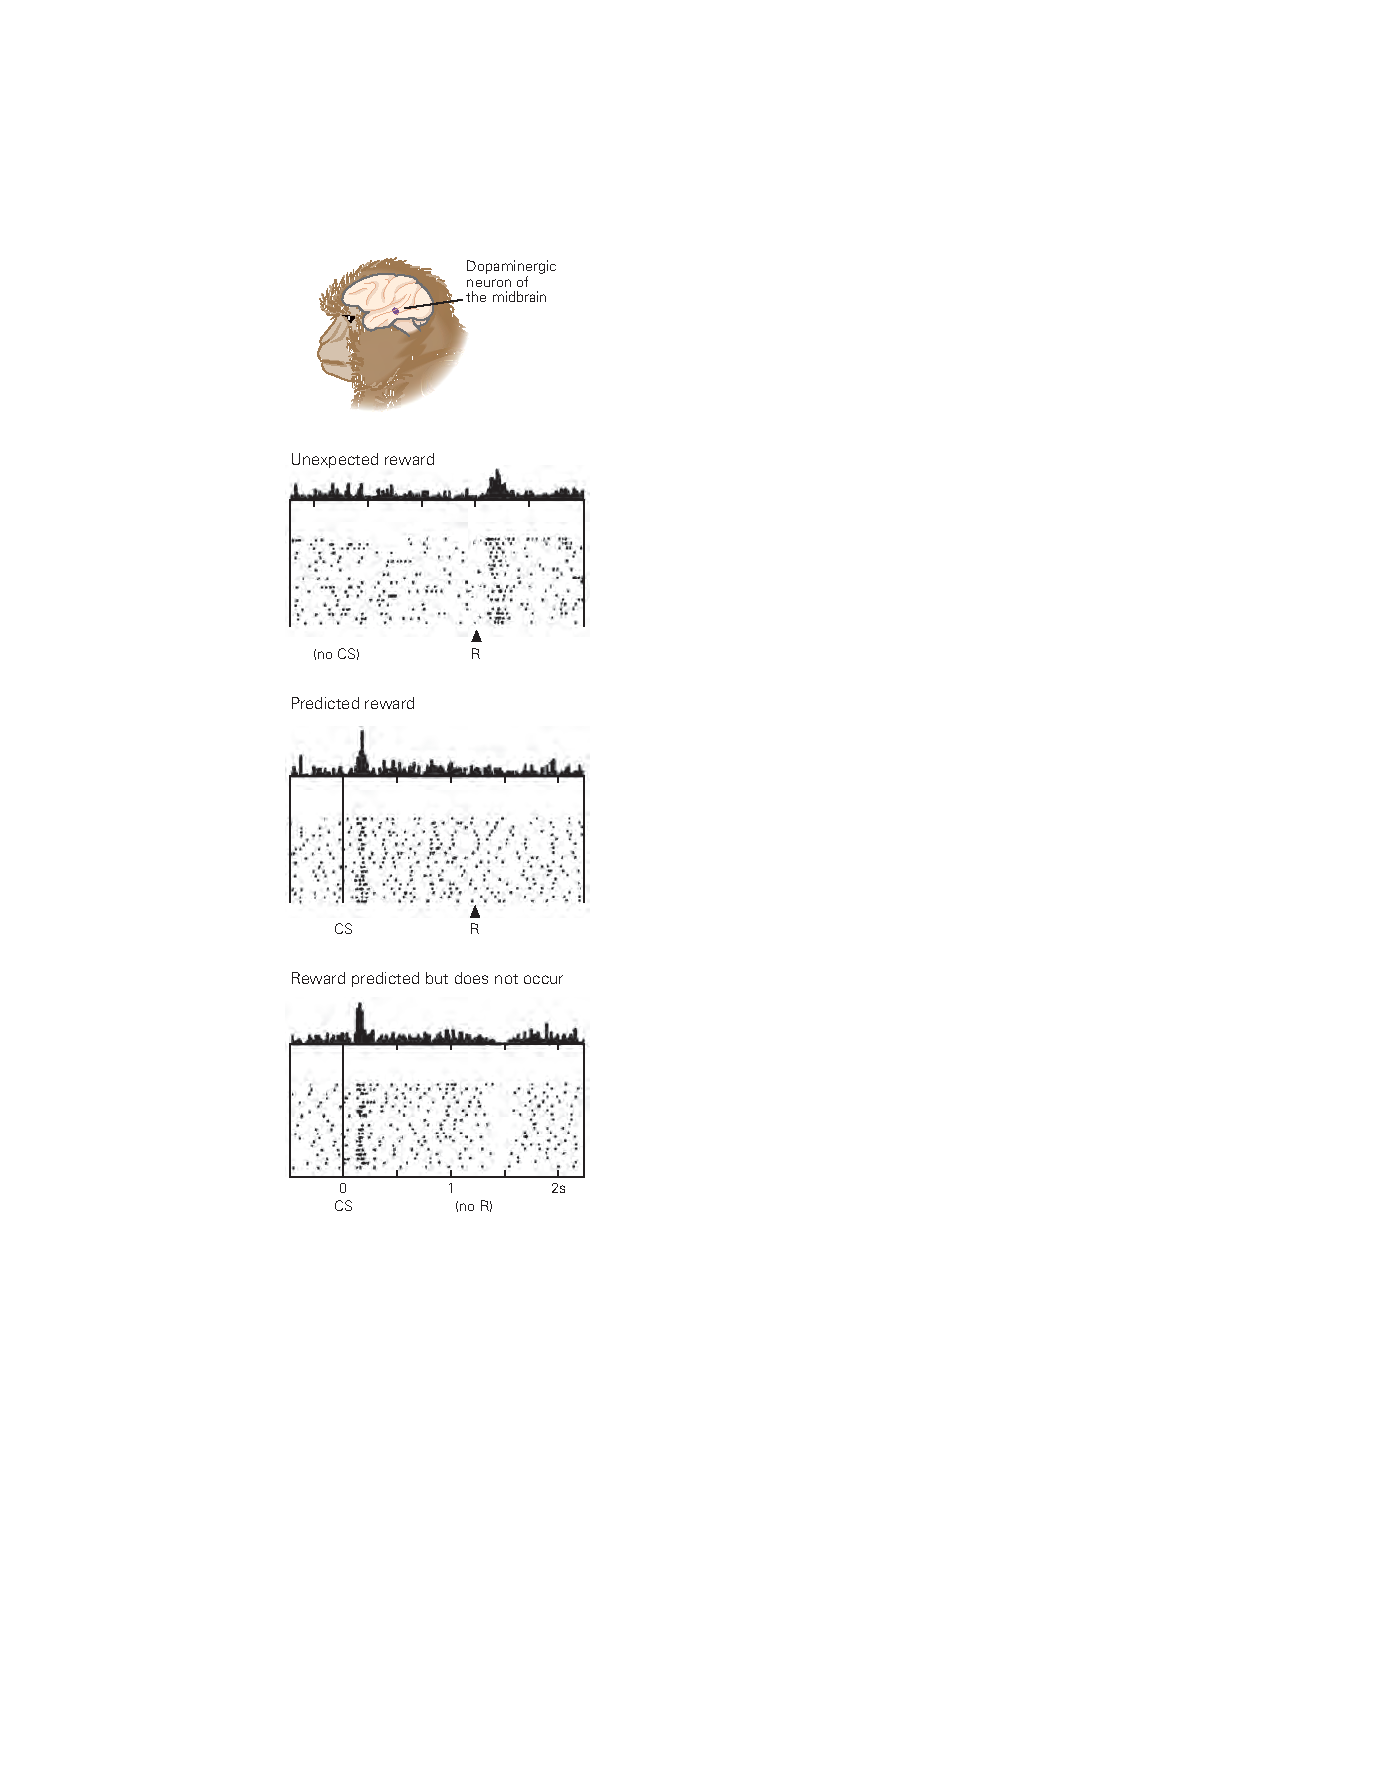
\includegraphics[width=0.46\linewidth]{chap43/fig_43_2}
	\caption{多巴胺能神经元报告奖赏预测错误。
		图表显示了清醒、活跃的猴子中脑多巴胺能神经元记录的放电率。
		上图:一滴甜味液体在没有警告的情况下被送到猴子面前。
		\textit{意外的奖励}在神经元中引起反应。
		因此,奖励可以被解释为奖励预测中的正误差。
		中间:猴子已接受\textit{条件刺激}预测奖励的训练。
		在此记录中,奖励根据预测发生并且不会在神经元中引起反应,因为奖励的预测没有错误。
		神经元被第一次出现的预测刺激激活,而不是被奖励激活。
		底部:条件刺激预测未能发生的奖励。
		多巴胺能神经元在奖赏发生时表现出放电减少\cite{schultz1997neural}。}
	\label{fig:43_2}
\end{figure}


这些观察结果表明,前脑中多巴胺的释放不是一种愉悦信号,而是一种预测误差信号。
多巴胺的爆发意味着未曾预料到的奖励或与奖励相关的刺激;
停顿表示预测的奖励低于预期或不存在。
如果奖励与环境线索所预期的一样,多巴胺能神经元将保持其强直(基线)放电率。
因此,多巴胺释放的改变被认为会改变未来对刺激的反应,以最大限度地提高获得奖励的可能性,并最大限度地减少无结果的追求。
对于自然奖励,例如舒尔茨实验中猴子饮用的甜汁,一旦学习到奖励的环境线索,多巴胺能神经元放电就会恢复到基线水平。
舒尔茨将此解释为只要环境没有任何变化,就没有更多需要学习的东西,因此不需要改变行为反应。


在人体中使用功能性磁共振成像的实验提供了进一步的证据,证明多巴胺能激动剂和拮抗剂调节奖赏学习和伏隔核中的\textit{血氧水平依赖}信号。
然而,在一些实验中,缺乏多巴胺合成基因的小鼠仍然可以学习在哪里可以找到糖或可卡因奖励,这表明并非所有形式的奖励学习都需要多巴胺。
此外,接受苯丙胺以在更长时间间隔内提高突触前多巴胺水平的啮齿动物表现出增强的“想要”行为(即,在存在预测蔗糖奖励的巴甫洛夫线索的情况下增加响应)。


这些考虑导致一些研究人员认为多巴胺具有比通过提供预测错误信号简单地驱动强化学习更广泛的作用。
事实上,最近的几项研究表明,中脑多巴胺能神经元不同亚群的反应特性存在相当大的差异。
一些神经元被奖赏和厌恶刺激同时激活,而另一些神经元倾向于被两种类型的刺激之一激活,还有一些神经元表现出相反的反应(被奖赏激活并被厌恶刺激抑制)。
有一些证据表明,这些神经元差异与多巴胺能神经元亚群之间的传入输入和传出投射的差异有关。
理解这种多巴胺信号复杂混合的确切作用:在学习、驱动目标导向行为中,尤其是在更复杂的学习形式中,这些学习形式涉及更长的时间尺度的动作序列以获得遥远的奖励,仍然是一个活跃的研究领域。


与自然奖赏不同,无论服用上瘾药物的频率如何,都会导致奖赏回路中的多巴胺释放,而且这种释放的幅度通常大于自然奖赏时所见的多巴胺,即使药物不再产生主观愉悦,多巴胺也会释放。
对大脑来说,服用成瘾药物可能总是发出“好于预期”的信号,并以这种方式继续影响行为,以最大限度地寻求药物和吸毒。
如果这个想法是正确的,它可能会解释为什么药物寻求和消费会变得强迫性的,以及为什么上瘾者的生活越来越专注于吸毒而忽略了所有其他追求。



\section{吸毒成瘾是一种病态的奖赏状态}

吸毒成瘾是一种慢性的、有时甚至是致命的综合症,其特征是尽管有严重的负面后果,如身体疾病和无法在家庭、工作场所或社会中发挥作用,但仍会强迫性地寻求和吸毒。
许多吸毒者都知道他们成瘾的破坏性,但尽管进行了多次治疗尝试,仍无法改变他们的成瘾行为。


吸毒成瘾的一个有趣特征是所有化学物质中只有一小部分会导致这种综合症。
这些所谓的滥用药物没有共同的化学结构,它们通过与大脑中不同的蛋白质靶标结合来产生作用。
相反,这些不同的物质每一种都会导致类似的成瘾行为综合症,因为它们的行为集中在控制奖赏和动机的大脑回路上(图~\ref{fig:43_3})。


\begin{figure}[htbp]
	\centering
	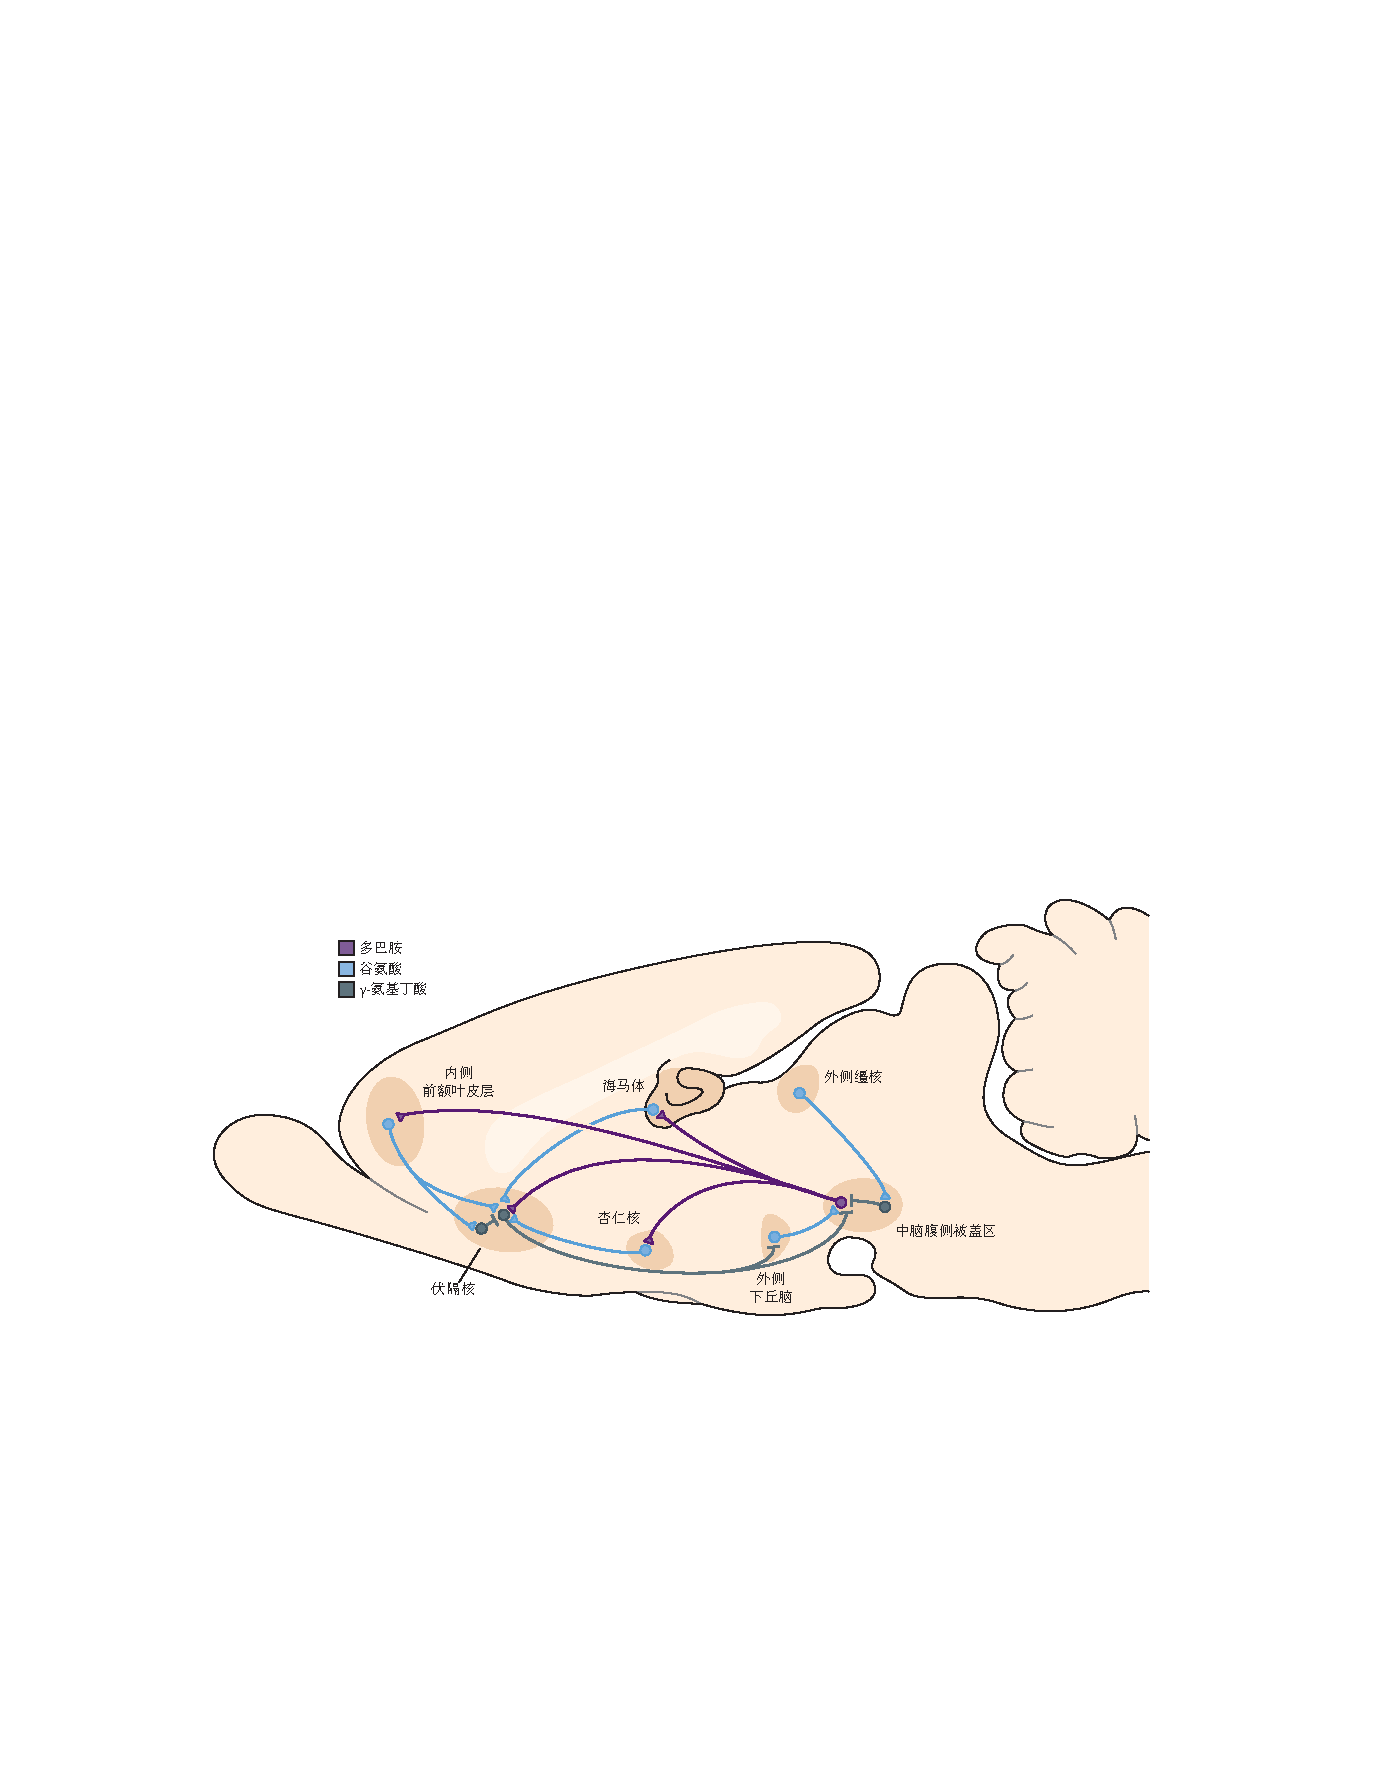
\includegraphics[width=1.0\linewidth]{chap43/fig_43_3}
	\caption{大脑奖励回路。
		啮齿动物大脑中主要的多巴胺能、谷氨酸能和$\gamma$-氨基丁酸能连接进出\textit{腹侧被盖区}和\textit{伏隔核}的示意图。
		主要奖励回路包括从\textit{腹侧被盖区}到\textit{伏隔核}的多巴胺能投射。
		\textit{腹侧被盖区}投射释放多巴胺以响应与奖励相关的刺激(在某些情况下与厌恶相关的刺激)。
		也有从\textit{伏隔核}到\textit{腹侧被盖区}的\textit{$\gamma$-氨基丁酸}能投射,一些在直接通路中支配\textit{腹侧被盖区},一些在间接通路中通过干预腹侧苍白球中的\textit{$\gamma$-氨基丁酸}能神经元支配\textit{腹侧被盖区}(未显示)。
		\textit{伏隔核}还包含多种类型的中间神经元。
		\textit{伏隔核}从\textit{内侧前额叶皮层}、\textit{海马体}、\textit{外侧缰核}和\textit{杏仁核}等区域接收来自谷氨酸能单突触回路的密集神经支配。
		\textit{腹侧被盖区}从杏仁核和前额叶皮层以及几个使用递质乙酰胆碱(未显示)的脑干核团接收此类输入。
		它还接收下丘脑外侧神经元的肽能末端以及其他输入。
		这些不同的输入控制与奖励相关的感知和记忆的各个方面\cite{russo2013brain}。}
	\label{fig:43_3}
\end{figure}


对这些行为的理解的进展在很大程度上是基于对实验室动物的研究,这些动物自我服用导致人类成瘾的相同药物。
事实上,当动物可以免费和无限制地使用这些药物时,一部分动物将失去对药物消耗的控制(这变得越来越不自愿),以牺牲进食和睡眠为代价,有些甚至会因过量服用而死亡。
药物自我给药和其他成瘾动物模型(方框~\ref{box:43_1})使得研究滥用药物产生初始奖赏效果的神经回路以及药物在该回路中诱导的分子和细胞适应成为可能 反复接触后会导致成瘾样综合症。
在过去十年中,这些对动物的研究,连同对人类成瘾者的大脑成像研究,提供了对成瘾过程越来越完整的看法。


\begin{proposition}[药物成瘾的动物模型] \label{box:43_1}
	
	\quad \quad 几种动物模型在理解成瘾性药物在反复暴露后如何产生急性奖励和成瘾样综合症方面发挥了重要作用。
	
	\quad \quad 药物自我管理
	
	\quad \quad 药物的增强作用可以在动物执行任务(例如,按下杠杆)以接受静脉内药物注射的实验中得到证明。
	除了研究这种行为的获得之外,科学家还评估了动物通过使用渐进比例程序来递送药物的难度,其中每个连续的药物剂量都需要越来越多的杠杆按压。
	
	\quad \quad 当动物停止自我给药时,就会达到所谓的断点。
	在药物自我给药停止或消失数周或数月后,动物会表现出类似复发的行为:
	它们会按下不再传递药物的刺激杆,以响应测试剂量的药物,先前与药物相关的线索(光线或音调)或压力。
	这些不同的自我管理行为被认为是人类成瘾的最佳验证模型。
	
	\quad \quad 条件性位置偏好
	
	\quad \quad 动物学会将特定环境与被动接触药物联系起来。
	例如,啮齿动物在盒子的一侧服用可卡因的时间比服用生理盐水的一侧要长。
	这种范式提供了药物奖励效力的间接测量,并证明了成瘾药物的强烈线索条件效应。
	
	\quad \quad 运动敏化
	
	\quad \quad 所有滥用药物在初次接触药物时都会刺激啮齿动物的运动,反复服用药物后会增加运动激活。
	由于介导对滥用药物的运动反应的神经回路与介导奖赏和成瘾的回路部分重叠,因此运动敏化提供了一个模型,用于研究慢性药物暴露过程中该回路的可塑性。
	
	\quad \quad 颅内自我刺激
	
	\quad \quad 动物会工作(例如,按下杠杆)将电流传递到大脑奖励回路的部分(见图~\ref{fig:43_1})。
	滥用药物会降低这种自我刺激的刺激阈值,这意味着在存在药物的情况下,动物会在控制条件下产生无效的刺激频率。
	
\end{proposition}



\subsection{所有滥用药物都以神经递质受体、转运体或离子通道为目标}

关于成瘾药物与神经系统的最初相互作用,人们已经了解很多。
实际上,与这些药物相互作用的所有蛋白质都已被克隆和表征(表~\ref{tab:43_1})。


\begin{table}[htbp]
	\caption{成瘾药物的主要类别} \label{tab:43_1} \centering
	\begin{tabular}{llll}
		\toprule
		类别 & 来源 & 分子靶标 & 示例 \\
		\midrule
		鸦片剂 & 罂粟 & $\mu$阿片受体(兴奋剂) & \makecell[l]{吗啡、美沙酮、氧可酮、\\海洛因、许多其他类} \\
		精神运动兴奋剂 & 古柯叶、合成 & 多巴胺转运体(拮抗剂) & \makecell[l]{可卡因、安非他命、\\甲基苯丙胺} \\
		大麻类 & 大麻 & 大麻素受体(兴奋剂) & 大麻 \\
		尼古丁 & 烟草 & 烟碱型乙酰胆碱受体(兴奋剂) & 烟草 \\
		乙醇 & 发酵 & \makecell[l]{$\gamma$-氨基丁酸$_A$受体(兴奋剂)、\\\makecell[l]{N-甲基-D-天冬氨酸型谷氨酸\\受体(拮抗剂)}\\和多个其他靶标} & 各种各样的饮料 \\
		类苯环利定毒品 & 合成 & \makecell[l]{N-甲基-D-天冬氨酸型谷氨酸\\受体(拮抗剂)} & 苯环利定 \\
		镇静剂/安眠药 & 合成 & $\gamma$-氨基丁酸$_A$受体(正变构调节剂) & \makecell[l]{巴比妥类药物、\\苯二氮平类药物} \\
		\bottomrule
	\end{tabular}
\end{table}


每一类滥用药物都会产生不同范围的急性行为影响,这与每一类作用于不同靶标并且这些靶标在整个神经系统和周围组织中具有不同表达模式的事实一致。
可卡因和其他精神兴奋剂正在激活并可能引起心脏副作用,因为它们的靶标(单胺转运蛋白)在支配心脏的外周神经中表达。
相反,阿片类药物是镇静剂和强效镇痛剂,因为它们的靶点(阿片受体)在睡眠和疼痛中枢表达。


然而,所有滥用药物都会敏锐地诱导奖赏和强化,这种共同作用反映了这样一个事实,即尽管药物的初始目标非常不同,但它们会对大脑的奖赏回路产生一些共同的功能影响(图~\ref{fig:43_4})。
这些共同的初始效应中最确定的是增加伏隔核中的多巴胺能神经传递,尽管是通过不同的机制。
例如,可卡因通过阻断位于腹侧被盖神经元末端的多巴胺再摄取转运蛋白产生这种效果,而阿片类药物通过抑制附近的\textit{$\gamma$-氨基丁酸能}中间神经元激活腹侧被盖区多巴胺神经元细胞体。


\begin{figure}[htbp]
	\centering
	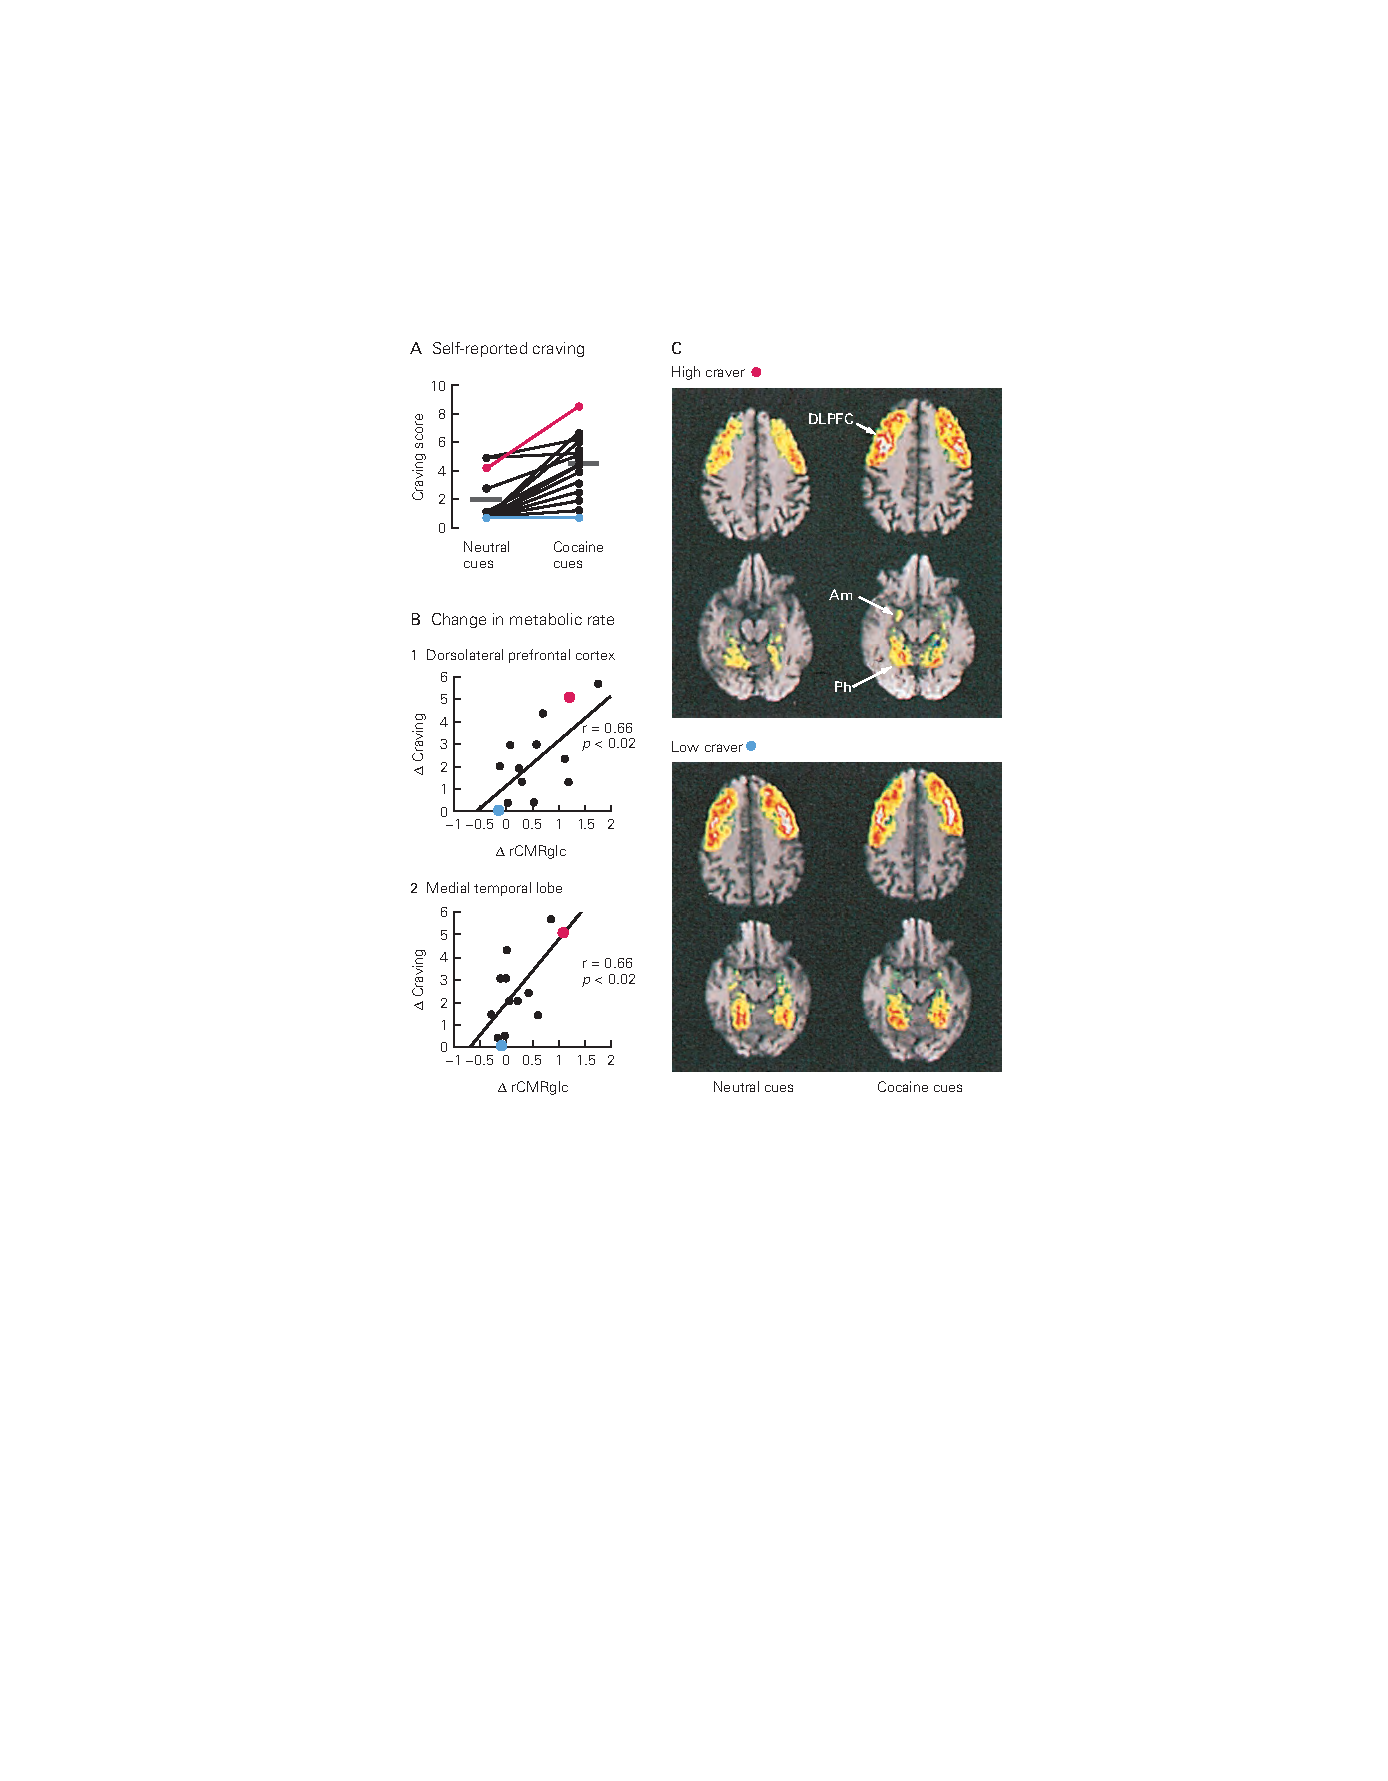
\includegraphics[width=0.8\linewidth]{chap43/fig_43_4}
	\caption{\textit{正电子发射断层成像}揭示了线索诱导的可卡因渴望的神经相关性\cite{grant1996activation}。
		\textbf{A.} 向受试者展示中性或与可卡因相关的线索,并询问:“在 1-10 的范围内,你如何评价你对可卡因的渴望或冲动?” 
		暴露于可卡因相关线索的平均渴望分数(水平条)明显高于暴露于中性刺激的平均渴望分数(水平条),尽管个体之间的反应程度差异很大。
		由红点和蓝点标识的两个主题分别代表高层和低层渴望。
		\textbf{B.} 自我报告的渴望的变化与暴露于可卡因相关线索期间背外侧前额叶皮层和内侧颞叶的代谢率变化相关。
		横坐标绘制了两个会话之间代谢率的差异(可卡因线索的活动减去中性线索的活动)。
		代谢率被测量为\textit{区域大脑葡萄糖代谢率}。
		纵坐标绘制了对“你对可卡因有渴望或冲动吗?”这个问题的平均回答之间的差异。
		在具有中性和可卡因相关线索的单独会话中。
		(每个环节持续 30 分钟,在每个环节中,问题被问了 3 次。)
		\textbf{C.} 当受试者报告对可卡因有渴望时,\textit{背外侧前额叶皮层}和两个内侧颞叶结构的代谢活动增加,\textit{杏仁核}和\textit{海马旁回}。
		代谢活动的伪彩色\textit{正电子发射断层成像}图像在空间上与高分辨率结构磁共振图像对齐。
		一名受试者的杏仁核和海马旁回的代谢率显著增加,该受试者报告在呈现可卡因相关线索(A 和 B 部分中的红点)期间渴望大幅增加。
		在报告暴露于可卡因相关线索(A 和 B 部分中的蓝点)时渴望没有增加的受试者中,这种效果并不明显。
		未显示背外侧前额叶皮层和内侧颞叶以外的代谢活动。}
	\label{fig:43_4}
\end{figure}


阿片类药物还通过独立于多巴胺的作用产生奖赏(例如,通过激活伏隔核神经元本身的阿片受体)。
所有其他滥用药物通过多巴胺依赖性和非依赖性机制(例如,内源性阿片类药物和大麻素信号传导的激活)的组合起作用,以对伏隔核神经元产生一些相同的功能影响。
重要的是,通过增加多巴胺能神经传递,所有这些药物也产生一些相同的功能效应,这些效应由多巴胺受体的激活介导,作用于腹侧被盖多巴胺神经元的许多其他投射目标(图~\ref{fig:43_3}),这些作用也有助于奖励和 在启动一些反复接触药物的有害行为时。



\subsection{反复接触滥用药物会导致持久的行为适应}

滥用药物的急性奖励行为不能解释成瘾。
相反,成瘾是由大脑对反复暴露于此类急性行为的适应所介导的。
该领域仍然存在两个主要问题:哪些特定适应介导了成瘾行为综合症,以及为什么有些人更容易上瘾?


我们知道在动物和人类中,所有滥用药物的成瘾风险中大约有 50\% 是遗传的,但赋予风险的特定基因在很大程度上仍然未知。
与大多数其他常见慢性病一样,成瘾的遗传风险非常复杂,反映了数百种遗传变异的综合作用,每一种变异的影响都非常小。
其他 50\% 的风险虽然尚未完全了解,但涉及许多环境因素,包括早年生活压力、终生压力和同伴压力。


从历史上看,通过一系列药理学术语描述了反复接触药物引起的适应。
耐受性是指以相同剂量重复给药后药物的作用减弱或需要增加剂量以产生相同的作用。
致敏作用,也称为反向耐受性,发生在重复给药相同剂量的药物会引起增强作用时。
依赖性被定义为一种适应性状态,它响应于重复给药而发展,并在戒断期间显露,戒断发生在停止吸毒时。
戒断症状因药物而异,包括与药物急性作用相反的作用。
许多不上瘾的药物都会出现耐受、致敏和依赖/戒断。
例如,两种用于治疗高血压的药物,$ \beta $-肾上腺素能拮抗剂普萘洛尔和$ \alpha $2-肾上腺素能激动剂可乐定,会产生强烈的依赖性,突然停药后会出现严重的高血压。


滥用药物在奖励和动机相关行为中引起耐受、敏感和依赖/戒断方面是独一无二的,这些行为导致成瘾综合症。
奖赏耐受性可以被视为对重复药物暴露做出反应的内源性奖赏机制的稳态抑制,是导致药物使用模式升级的一个因素。
动机依赖表现为早期戒毒期间出现的负面情绪(例如,抑郁和焦虑样)症状,并且还受抑制的内源性奖赏机制介导,是推动重新吸毒或复发的主要因素。
奖赏敏感化通常发生在较长的戒断期后,可触发复发以响应暴露于药物本身或与药物相关的线索(例如,与人在一起或在以前使用过药物的地方)。


有趣的是,由于药物的不同急性作用,一种给定的药物可以同时产生所有这些适应性:耐受性、致敏性和依赖性; 
这种现象强调了多种细胞类型和回路参与调节药物的整体作用。
神经科学家面临的主要挑战是确定特定类型的神经元和神经胶质细胞的变化(以及它们对回路功能的后续贡献),这些变化是由反复接触药物引起的,并介导定义成瘾状态的行为特征。



\subsection{通过重复药物暴露在大脑奖励区域诱导持久的分子适应}

大量文献表明,在动物模型中反复接触滥用药物会改变许多神经递质和神经营养因子、它们的受体和细胞内信号通路以及整个大脑奖赏回路中的转录调节蛋白的水平。
大多数这些变化无法在活体患者身上进行研究(只有少数神经递质和受体可以在患者脑部成像中进行评估),尽管对死后人类脑组织的研究正越来越多地用于验证动物模型的发现。
大多数报告的研究都集中在腹侧被盖区和伏隔核上,尽管越来越多的研究正在检查奖赏回路的其他部分。


最有力的实验结果可用于精神兴奋剂和阿片类药物,这可能是因为这些药物引起的变化比其他滥用药物的变化幅度更大。
这可能反映了精神兴奋剂和阿片类药物具有更大的内在成瘾性:与其他类别的滥用物质相比,在相同的暴露量下,更多的人会对这些药物上瘾。
然而,考虑到酒精、尼古丁和大麻成瘾对公共健康的主要影响,应该更多地关注这些药物。


下面,我们通过关注少数与动物模型中成瘾的特定行为特征有因果关系的药物诱导的适应来总结这一大量文献。
正如在下一节中将清楚的那样,当前的研究重点是将这些和许多其他分子变化与突触和回路适应相关联,这些变化也与成瘾有关。


\textit{环磷酸腺苷}-\textit{环磷酸腺苷应答元件结合蛋白}通路的上调

几种滥用药物会激活 $ G_i $ 蛋白连接的受体,例如 D2 多巴胺受体;
$ \mu $、$ \delta $ 和 $ \kappa $ 阿片受体;
和\textit{大麻素受体}。
这意味着,在一定程度上,许多滥用药物会激活 $ G_i $ 蛋白相关的信号通路,在伏隔核和其他靶神经元中产生诸如抑制腺苷酸环化酶(第~\ref{chap:chap14}~章)等作用。


过去二十年的工作已经确定,在反复接触后,受影响的神经元通过上调\textit{环磷酸腺苷}通路来适应这种持续抑制,包括诱导腺苷酸环化酶和蛋白激酶 A 的某些同种型。
重复药物 暴露同样会诱导转录因子\textit{环磷酸腺苷应答元件结合蛋白}的上调,\textit{环磷酸腺苷应答元件结合蛋白}通常由\textit{环磷酸腺苷}通路激活。
\textit{环磷酸腺苷}-\textit{环磷酸腺苷应答元件结合蛋白}通路的这种上调可以看作是耐受性和依赖性的分子机制:
尽管存在药物(耐受性和依赖性),但它恢复了这些通路的正常活性,并且当药物被去除时,上调的通路不受反对, 引起通路的异常高活性(退出)(图~\ref{fig:43_5})。
事实上,在动物模型中,伏隔核神经元中 \textit{环磷酸腺苷}-\textit{环磷酸腺苷应答元件结合蛋白}通路的上调已被证明可以介导奖赏耐受和动机依赖以及退缩。


\begin{figure}[htbp]
	\centering
	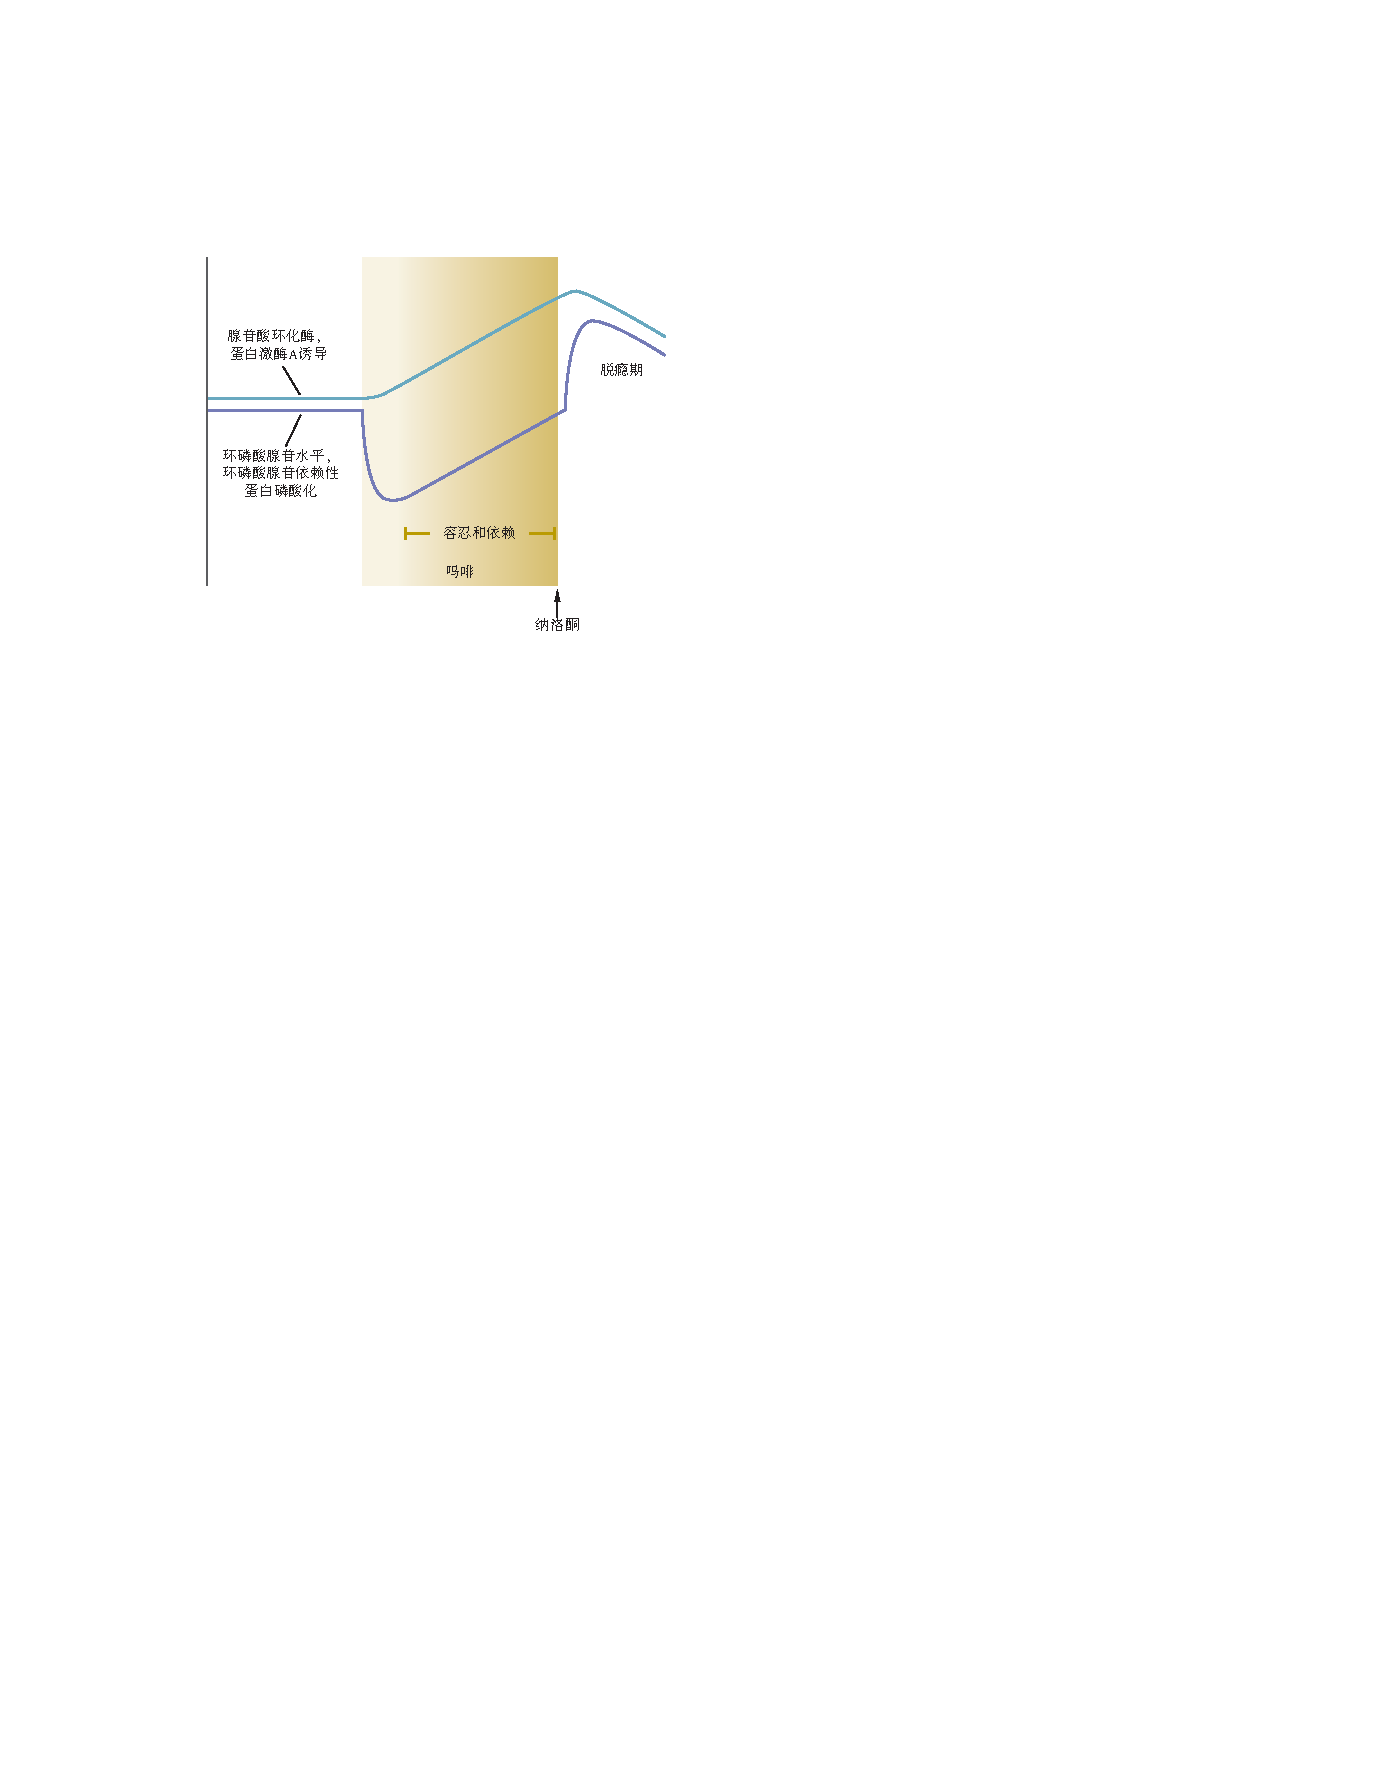
\includegraphics[width=0.6\linewidth]{chap43/fig_43_5}
	\caption{\textit{环磷酸腺苷}-\textit{环磷酸腺苷应答元件结合蛋白}通路的上调是药物耐受性和依赖性的分子机制。
		吗啡或其他 $\mu$ 阿片受体激动剂可急性抑制脑奖赏神经元中\textit{环磷酸腺苷}通路的功能活性,例如,\textit{环磷酸腺苷}或\textit{蛋白激酶A}的细胞水平依赖性底物磷酸化表明,例如 作为\textit{环磷酸腺苷应答元件结合蛋白}。
		随着持续的药物暴露(阴影),\textit{环磷酸腺苷}-\textit{环磷酸腺苷应答元件结合蛋白}通路的功能活性逐渐上调,并在药物去除后增加远高于控制水平(例如,通过施用 μ 阿片受体拮抗剂\textit{纳洛酮})。 \textit{环磷酸腺苷}-\textit{环磷酸腺苷应答元件结合蛋白}通路功能状态的这些变化是通过腺苷酸环化酶和\textit{蛋白激酶A}的诱导以及\textit{蛋白激酶A}底物如\textit{环磷酸腺苷应答元件结合蛋白}的激活来介导的,以响应重复给药。
		这些蛋白质的诱导解释了在慢性药物暴露(耐受性和依赖性)期间观察到的 \textit{环磷酸腺苷}-\textit{环磷酸腺苷应答元件结合蛋白}通路功能活性的逐渐恢复,以及在去除药物(戒断)后观察到的 \textit{环磷酸腺苷}-\textit{环磷酸腺苷应答元件结合蛋白}通路活性升高的原因。
		首先针对阿片类药物进行了证明,类似的规定也出现在对其他几种类型的滥用药物的反应中\cite{trimble2002molecular}。}
	\label{fig:43_5}
\end{figure}


诱导 $\Delta$FosB

$\Delta$FosB 是 Fos 转录因子家族的成员。
它是通过可变剪接生成的 FosB 基因的截短产物。
与 Fos 家族的所有其他成员相比,Fos 家族的所有其他成员都在响应神经活动或细胞信号传导中的许多扰动时被快速和短暂地诱导,而 $\Delta$FosB 仅在刺激的初始呈现时被轻微诱导。
然而,随着反复药物暴露,$\Delta$FosB 因其异常的稳定性而在神经元中积累,这在所有 Fos 家族蛋白中都是独一无二的。


在反复接触几乎任何滥用药物(包括可卡因和其他精神运动兴奋剂、鸦片制剂、尼古丁、乙醇、大麻素和苯环利定)后,伏隔核和其他几个大脑奖赏区的神经元就会出现这种现象。
最近涉及在成年小鼠伏隔核中选择性表达或敲低 $\Delta$FosB 的研究提供了直接证据,表明 $\Delta$FosB 的诱导介导了奖励致敏,包括增加药物自我给药和复发。
这是对滥用药物的共同适应的又一个例子,它导致许多滥用药物共有的成瘾方面。


\textit{环磷酸腺苷应答元件结合蛋白}和 $\Delta$FosB 是许多与药物成瘾有关的转录因子中的两个。
正在进行的研究侧重于表征染色质调节机制,这些因子通过这些机制协同调节受影响神经元和胶质细胞中特定基因的表达。
还正在进行工作以了解这些目标基因如何通过改变涉及突触、细胞和回路功能的蛋白质的表达来驱动它们相关的行为异常(图~\ref{fig:43_6})。


\begin{figure}[htbp]
	\centering
	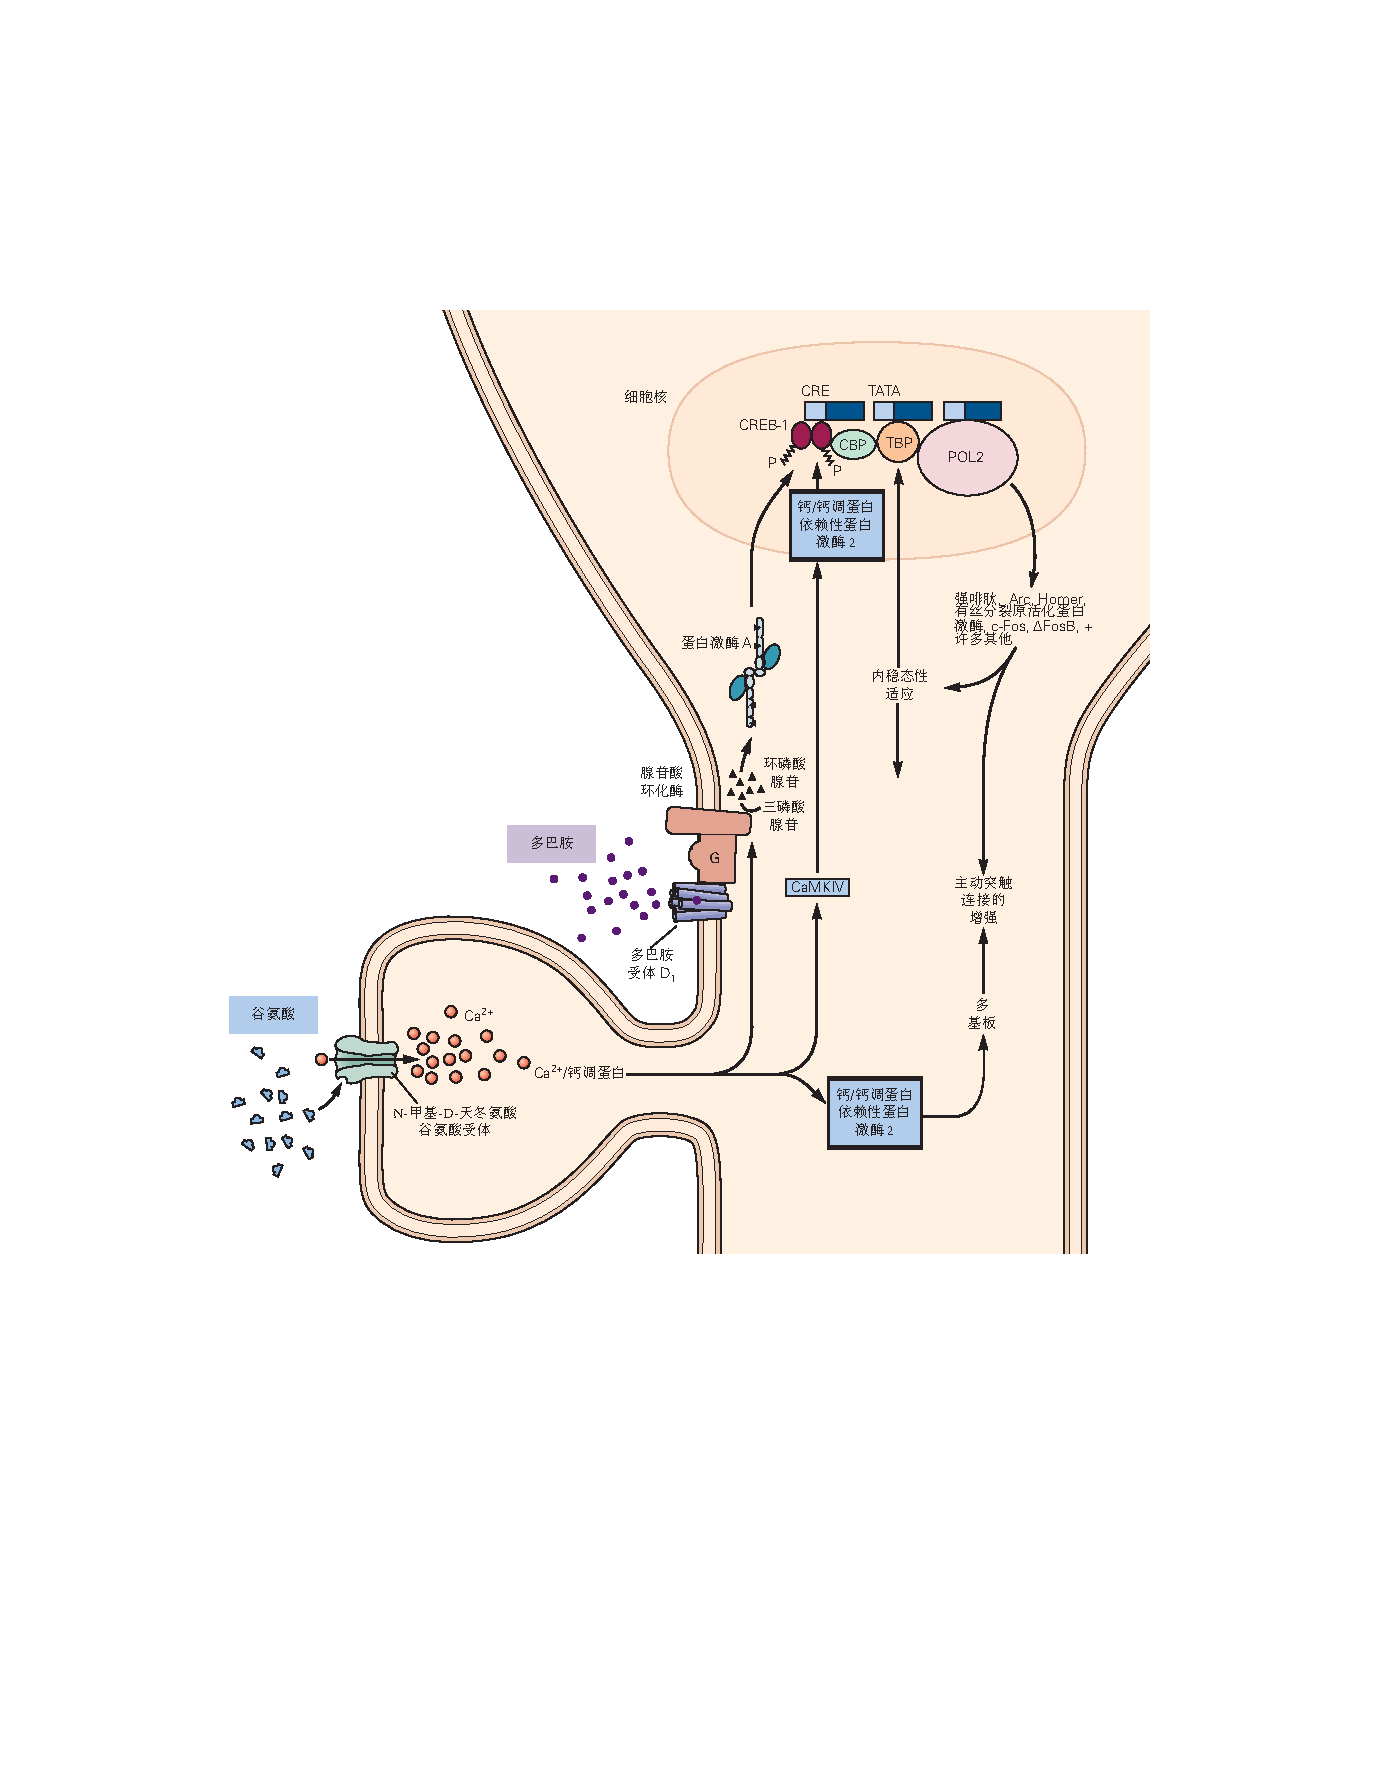
\includegraphics[width=0.98\linewidth]{chap43/fig_43_6}
	\caption{多巴胺和谷氨酸激活的细胞内信号通路与药物成瘾有关。
		\textit{N-甲基-D-天冬氨酸}型谷氨酸受体允许 \ce{Ca^2+} 进入,从而结合钙调蛋白。
		\ce{Ca^2+}/钙调蛋白复合物激活两种类型的 \ce{Ca^2+}/钙调蛋白依赖性蛋白激酶,细胞质中的\textit{钙/钙调蛋白依赖性蛋白激酶 2}和细胞核中的\textit{钙/钙调蛋白依赖性蛋白激酶 4}。
		某些多巴胺受体激活刺激性 G 蛋白,后者又激活腺苷酸环化酶以产生\textit{环磷酸腺苷}。
		\textit{环磷酸腺苷}依赖性\textit{蛋白激酶A}催化亚基可以进入细胞核。一旦在细胞核中被激活,\textit{蛋白激酶A}和\textit{钙/钙调蛋白依赖性蛋白激酶 4}都会磷酸化,从而激活\textit{环磷酸腺苷应答元件结合蛋白}。
		\textit{环磷酸腺苷应答元件结合蛋白}募集\textit{环磷酸腺苷应答元件结合蛋白}和许多其他染色质调节蛋白,从而激活许多基因的\textit{核糖核酸}聚合酶 II 依赖性转录,从而产生可以改变细胞功能的蛋白质。
		Arc 和 Homer 位于突触区域;
		\textit{有丝分裂原活化蛋白}是控制许多细胞过程的蛋白激酶;
		Fos和$\Delta$FosB是转录因子;
		强啡肽是一种内源性阿片肽。
		这些蛋白质被认为有助于对过度多巴胺刺激的稳态反应以及与记忆形成相关的突触的形态和功能变化。}
	\label{fig:43_6}
\end{figure}



\subsection{持久的细胞和回路适应调解吸毒成瘾状态的各个方面}

反复接触滥用药物可以通过两种主要方式改变神经回路。一种称为全细胞或稳态可塑性的机制涉及改变神经细胞的内在兴奋性,最终会改变它所属的更大回路的功能。
很容易想象大脑奖赏回路中神经元的全细胞可塑性如何调节奖赏耐受性、敏感性、依赖性和戒断性等方面。


另一种机制是突触可塑性,其中特定神经元之间的连接得到加强或减弱。
这些特定于突触的适应可以调节涉及适应不良记忆的成瘾特征,例如药物暴露与许多环境线索相关联的记忆。
这种病态的学习和记忆会以牺牲自然奖励为代价,使个体越来越专注于药物。
迄今为止,该领域的大部分注意力都集中在突触可塑性上。


\textit{突触可塑性}

正如本书其他地方所讨论的,谷氨酸能突触中描述了两种主要形式的突触可塑性:
\textit{长时程抑制}和\textit{长时程增强}。
在过去的二十年里,这两种适应的分子基础已经建立,在整个神经系统中出现的\textit{长时程抑制}和\textit{长时程增强}的几种不同亚型中的每一种都具有不同的机制。
我们现在知道,几种类型的滥用药物,特别是精神运动兴奋剂和阿片类药物,会导致大脑奖励回路中特定类别的谷氨酸能突触发生\textit{长时程抑制}和\textit{长时程增强}样变化,迄今为止的大部分工作都集中在腹侧被盖区和伏隔核。


伏隔核的变化显示出有趣的时间依赖性适应作为药物戒断的函数。
在早期戒断点(几小时到几天),伏隔核神经元上的谷氨酸能突触显示\textit{长时程抑制}样变化,在较长时间的戒断后(几周到几个月)演变成\textit{长时程增强}样变化。
伏隔核中药物诱导的\textit{长时程抑制}和\textit{长时程增强}样适应涉及与其他大脑区域(主要是海马体和大脑皮层)相似的形态学变化,其中\textit{长时程抑制}和\textit{长时程增强}与个体树突棘的形态学变化相关。
在早期戒断期间,\textit{长时程抑制}样反应与不成熟的细树突棘数量增加同时发生,而在后期戒断期间,\textit{长时程增强}样反应与成熟蘑菇状棘的数量增加同时发生。
这些发现表明,重复吸毒会通过诱导所谓的沉默突触(第~\ref{chap:chap54}~章)削弱伏隔核神经元的某些谷氨酸能突触,其中一部分突触会在长时间停药期间得到加强。


这些进展现在定义了几个正在进行的调查。
我们需要了解哪些特定的谷氨酸能连接受到影响,以及这些变化如何导致成瘾的行为特征。
我们需要定义这种依赖于时间的突触可塑性的分子基础,它部分是通过转录机制和许多蛋白质表达水平的改变来介导的,包括谷氨酸受体、突触后密度蛋白、调节肌动蛋白细胞骨架的蛋白质等 上(图~\ref{fig:43_6})。
此外,我们需要在腹侧被盖区和伏隔核之外的其他几个与奖励相关的大脑区域检查药物诱导的谷氨酸能突触可塑性,这些区域在成瘾状态下变得腐败。
最后,我们需要了解反复接触滥用药物如何破坏整个回路中的抑制性\textit{$\gamma$-氨基丁酸}能突触传递。


\textit{全细胞可塑性}

与突触可塑性一样,药物诱导的全细胞可塑性的大多数例子都涉及腹侧被盖区和伏隔核。
例如,反复接触可卡因会增加伏隔核神经元的内在兴奋性,这有助于奖赏耐受性。
这种适应部分是由于\textit{环磷酸腺苷应答元件结合蛋白}介导的特定类型 \ce{K+} 通道的表达减少,从而将分子转录适应与神经活动改变和成瘾相关的行为异常联系起来。
反复接触阿片类药物也会增加腹侧被盖区多巴胺能神经元的内在兴奋性,但会阻碍多巴胺能向伏隔核的传递。
与反复接触可卡因一样,这种适应也是通过抑制某些 \ce{K+} 通道来调节的,并有助于奖赏耐受性。


\textit{回路可塑性}

先进的工具首次使跟踪清醒、活跃的动物大脑中特定神经细胞类型的活动成为可能,并通过实验操纵这些细胞的活动并研究行为后果(第~\ref{chap:chap5}~章)。
这使科学家能够定义特定大脑区域内神经元的精确集合,这些神经元在成瘾的生命周期中受到药物暴露的影响(从最初的药物暴露到强迫性药物消耗再到戒断和复发),并提供参与的因果证据,这些神经元和它们发挥作用的微回路。
这项工作开始定义各种谷氨酸能投射到伏隔核的不同作用(来自前额叶皮层、海马、杏仁核和丘脑),在控制伏隔核和更广泛的奖赏回路中的不同细胞类型以及产生不同的成瘾方面发挥的作用 -相关的行为异常。


虽然我们在本章中专门关注滥用药物的急性和慢性作用对行为神经控制的影响,但我们意识到这是过于简单化了。
正如第~\ref{chap:chap7}~章所讨论的,神经元功能受大脑中大量非神经细胞的复杂控制,包括星形神经胶质细胞、小神经胶质细胞、少突胶质细胞和内皮细胞。
越来越多的证据表明,这些细胞类型中的每一种都直接或间接地受到滥用药物的影响,并且这些非神经元行为也会影响药物暴露的长期行为后果。
需要将此类行为与滥用药物的神经元效应相结合才能全面了解成瘾。



\subsection{自然成瘾与药物成瘾和相同的生物学机制}

如前所述,大脑的奖励回路进化为激励个人追求自然奖励,如食物、性和社交互动。
正如吸毒成瘾者表现出对滥用药物的强迫性消费,一些人表现出对非药物奖励的强迫性消费(例如,强迫性暴饮暴食、购物、赌博、视频游戏和性行为),其行为后果与吸毒成瘾者观察到的非常相似。
该领域的一个有趣问题是,这些所谓的“自然成瘾”是否是由构成药物成瘾基础的一些相同的分子、细胞和回路适应介导的。


这些正常的愉悦行为可能会过度激活某些因遗传或非遗传因素而特别容易受到影响的个体的奖赏机制。
与药物一样,这种激活可能会导致动机的深刻改变,从而促进最初奖励行为的重复,尽管与由此产生的强迫行为相关的负面后果的影响。
由于动物模型的局限性(想象一下强迫性购物的小鼠模型!),研究自然成瘾的神经生物学基础要困难得多,尽管在开发此类范例方面正在取得进展。
无论如何,人类大脑成像研究支持这样一种观点,即对药物和行为奖励的成瘾与大脑奖励回路的类似失调有关(图~\ref{fig:43_3})。



\section{要点}

1. 动机状态驱动寻求奖励或抵御或避免厌恶刺激的行为。
动机状态本身由各种内部和外部变量决定。
内部变量包括生理状态和认知状态。
外部变量包括具有先天奖励或厌恶特性的刺激,尽管这些特性的动机意义可能会被内部变量修改。


2. 奖励是可取的对象、刺激或行动。
奖励往往会引发驱动接近行为的动机状态。
奖励可以在短期内满足监管需求,但也可以来自实现长期目标的复杂行为序列。


3. 大脑中奖励相关回路的关键组成部分包括多巴胺能神经元和多巴胺能神经元靶向的大脑区域,例如伏隔核、腹侧苍白球、杏仁核、海马体和部分前额叶皮层。
然而,多巴胺本身并不能解释享乐体验。 


4. 许多多巴胺能神经元表现出生理反应特性,表明它们传达预测错误信号,当发生比预期更好的事情时会增强活动。
这种类型的信号可以在不同形式的强化学习中发挥关键作用,学习将刺激或行动与奖励联系起来。
然而,最近的研究表明,多巴胺能神经元的反应异质性比以前认为的要多,包括对厌恶刺激的反应。
这种异质性及其对神经回路功能的复杂影响仍然是活跃的研究领域。


5. 吸毒成瘾可以定义为不顾身体健康或职业和社会功能的负面影响而强迫性地寻求和服用药物。
成瘾的风险大约有 50\% 是遗传的,有数百个基因,每个基因对这种遗传性的影响都非常小。
重要的非遗传风险因素包括不良生活事件史。


6. 滥用药物仅占已知化合物的一小部分。
这些药物在化学上是多种多样的,每种类型最初作用于不同的蛋白质靶标。
然而,这些药物可以诱发常见的行为综合症,因为它们对这些目标的作用集中在对中脑多巴胺能神经元或其投射区域(如伏隔核)产生类似的功能影响。


7. 成瘾需要反复接触滥用药物。
这种反复接触通常伴随着耐受、敏感和依赖/退缩。
虽然许多未滥用的药物可以产生耐受性和依赖性/戒断反应,但滥用药物在产生这些适应性以及激励和奖励状态的敏感性方面是独一无二的。


8. 药物成瘾的适应部分是通过基因表达的持久变化来调节的,这会导致神经元内在活动的改变以及大脑奖赏回路中突触接触的结构和功能改变。


9. 当前研究的一个重要目标是了解无数的分子变化如何汇总成为神经和突触功能特定变化的基础。
同样,重要的是要了解这些神经和突触变化如何结合起来改变大脑更大的奖赏相关回路的功能,从而调节定义成瘾状态的特定行为异常。


10. 这种对成瘾的分子、细胞和回路机制的描述将需要更多地关注发生某些药物诱导适应的特定细胞类型(神经元和非神经元)以及受这些适应影响的奖赏途径中的特定微回路。


11. 一部分人对非药物奖励(如食物、赌博和性)表现出类似成瘾的行为异常。
有证据表明,这种所谓的自然成瘾是由涉及药物成瘾的相同大脑回路介导的,还涉及一些常见的分子和细胞异常。 


12. 这些考虑突出了需要更多地了解药物成瘾的精确分子、细胞和回路基础。
尽管如此,我们对大脑的奖赏回路以及回路中的个体突触和细胞如何因药物暴露而改变,从而破坏回路功能并篡夺正常的奖赏和联想记忆系统的不断深入的理解提供了一个令人信服的概念,即上瘾者会发生什么 脑。

